\documentclass{article}
\usepackage[utf8]{inputenc}
\usepackage{graphicx}

\title{Tugas Besar Database II \\
Aplikasi Klinik Dahlia}
\begin{figure}
\begin{center}
    
\includegraphics[width=6cm]{poltekpos.jpg}
\end{center}
\end{figure}
\author{Annisa Khairani Febrianti}
\date{1184071}

\begin{document}

\maketitle

\section{Membuat Aplikasi Pada Oracle Express}
\subsection{Pengertian Oracle APEX}
 Application Express(Oracle Apex), dulu disebut dengan HTTP DB yang artinya suatu aplikasi database yang berbasis web yang digunakan dalam database oracle. Oracle Apex ini mudah dipakai hanya menggunakan dengan web browser saja dan proses pemrograman yang sederhana, serta mengembangkan suatu ilmu dan kemampuan dengan aplikasi secara aman dan cepat.Application Express adalah suatu alat yang digunakan untuk membangun sebuah aplikasi web-based. Selain itu Oracle Application Express tidak membutuhkan perangkat lainnya untuk mengembangkan, menyebarkan serta menjalankan Aplikasi, karena di dalam Oracle Application Express telah menyediakan tiga alat utama. Tiga alat utama ini memiliki Kegunaan yang penting di dalam Oracle Application Express:
\begin{enumerate}
    \item Application Builder : Membuat aplikasi, melihat aplikasi, mengimport aplikasi, mengatur service, mengatur user aplikasi dan memantau aktifitas yang di lakukan pengguna.
    \item SQL Workshop : Membuat tabel dan komponennya (menggunakan kode PL-SQL secara manual maupun otomatis), melihat struktur tabel dan komponennya, mengimpor dan mengekspor script. 
    \item  Utilitas : Melihat suatu report table dan komponen history aplikasi.
\end{enumerate}
\newpage \section{Langkah-langkah membuat aplikasi pada Oracle APEX}
\begin{enumerate}
    \item Pertama-tama kita install terlebih dahulu Oracle Apex atau kamu juga dapat membuka oracle APEX di browser.
\par Catatan jika kamu menggunakan oracle apex yang online, pertama-tama kamu harus menginstall oracle apex kemudian ikuti langkah-langkah penginstalan dengan benar. Sehingga aplikasi tersebut dapat digunakan dengan baik. Setelah itu kamu akan diminta untuk mengisi suatu form login pendaftaran jika kamu belum memiliki akun oracle apex offline. Setelah selesai mengisi proses pendaftaran kamu akan masuk ke akun yang telah dibuat dengan memasukkan username dan password yang telah kamu buat. Setelah itu kita membuat workspace baru dengan cara pilih application express pada database user kemudian kita pilih create new,lalu kita isi Database username,Application express username,Password,dan confirm password. Setelah selesai kemudian kita pilih create workspace.Tetapi jika kalian sudah mempunyai workspace maka kita pilih already have account? kemudian kita login here pada button sebelah kanan. Setelah selesai kita dapat menggunakan oracle apex untuk membuat suatu query,aplikasi dan lain lain pada aplikasi oracle apex.
\end{enumerate}
\begin{figure} [h]
\centerline{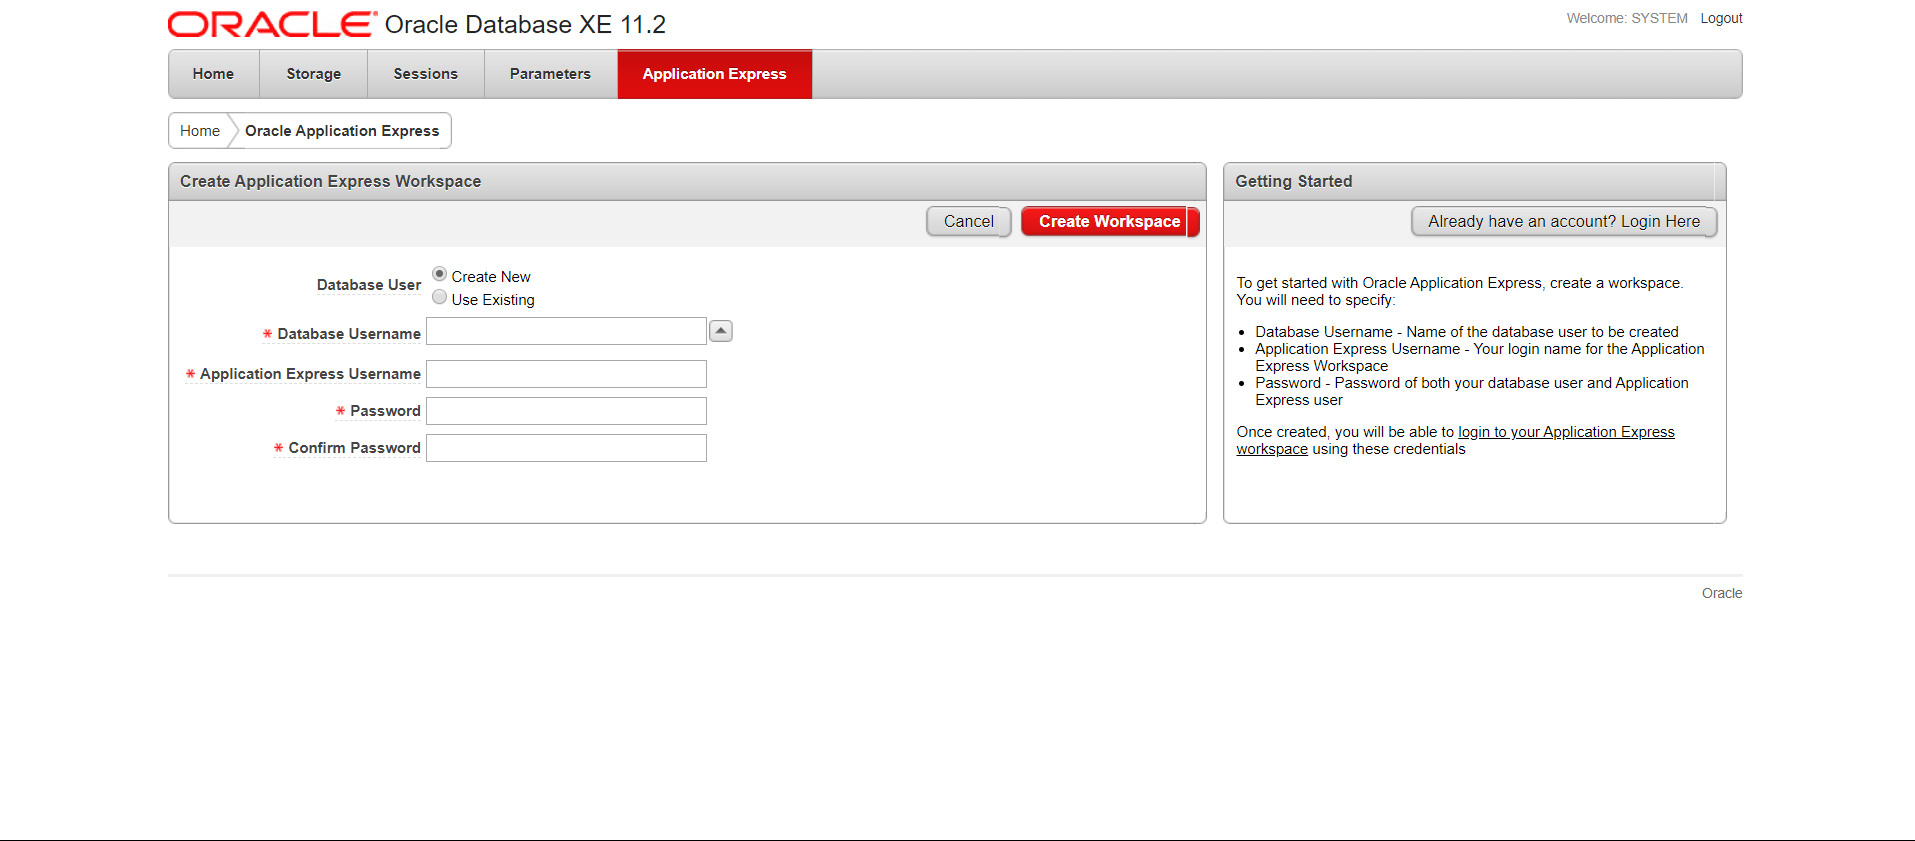
\includegraphics[width=10cm]{figure/oracle.PNG}}
\end{figure}
\newpage \par Catatan jika kamu ingin menggunakan Aplikasi Apex Online kita dapat mengunjungi link nya tersebut yaitu https://apex.oracle.com/en
\begin{figure} [h]
\centerline{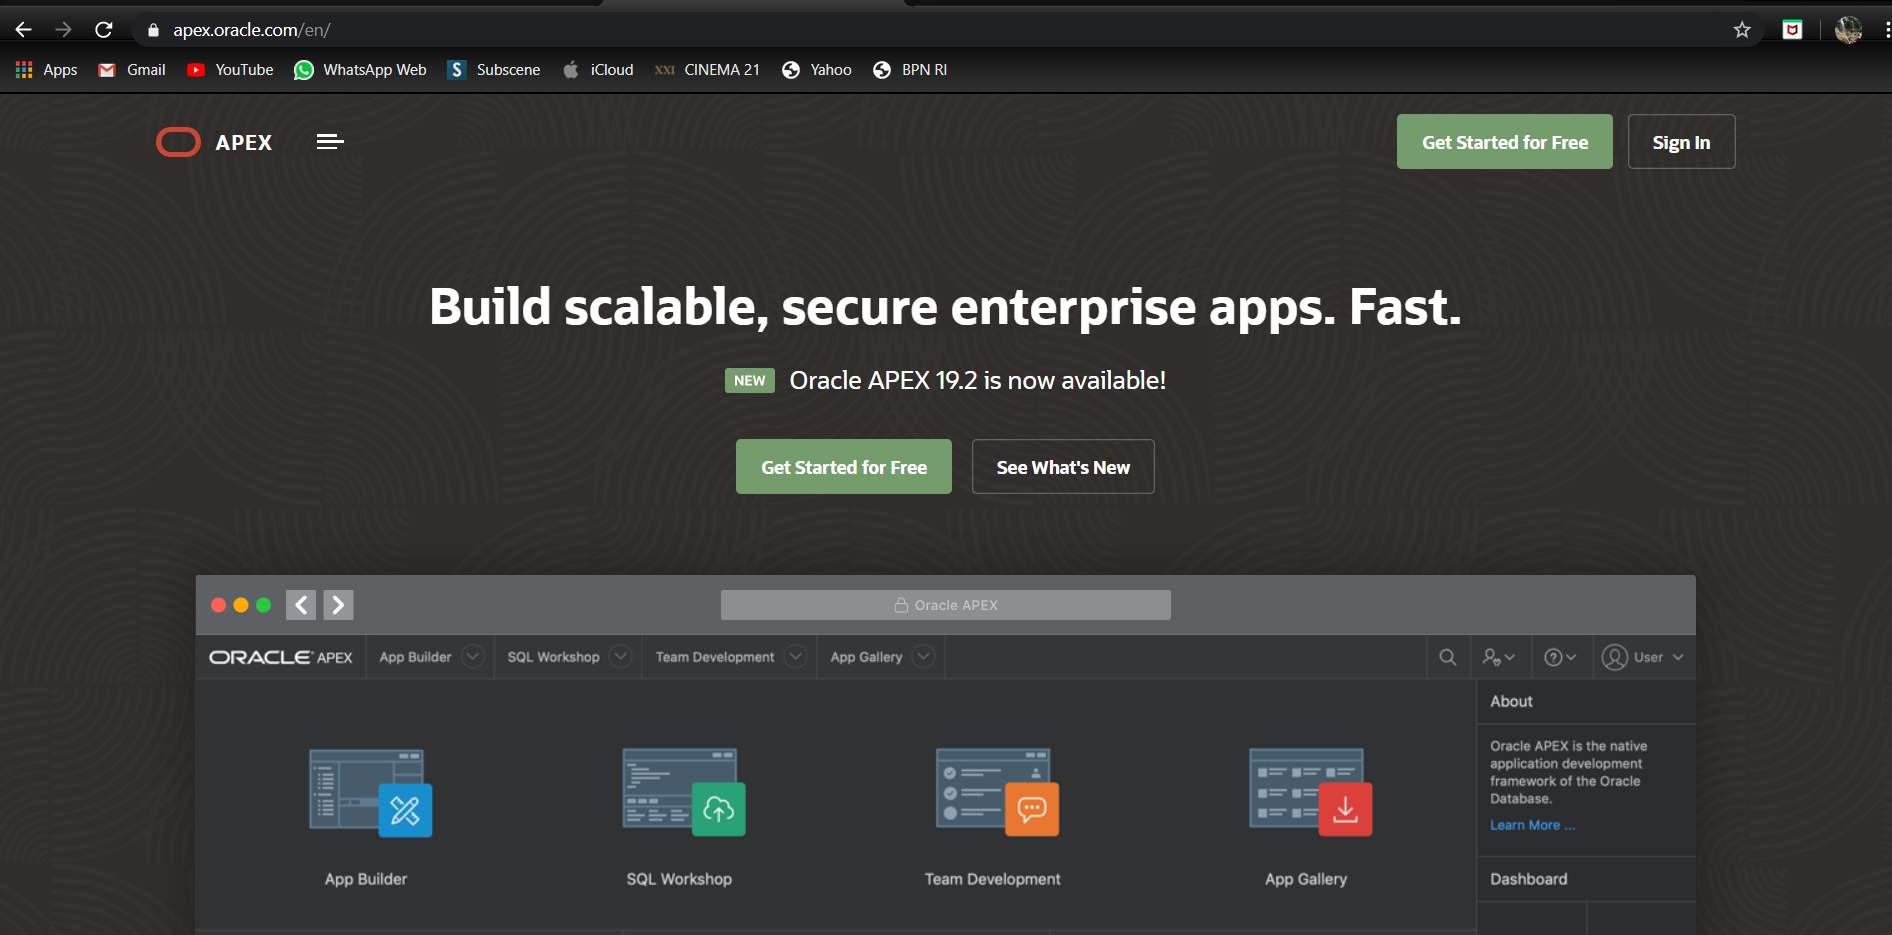
\includegraphics[width=10cm]{figure/apex1.PNG}}
\end{figure}
\subsection{Setelah kita masuk ke link aplikasi tersebut, ikuti langkah-langkah dibawah ini:}
\begin{enumerate}
    \item Pertama-tama kita pilih button Sigin terlebih dahulu, kemudian jika kalian sudah memiliki worskpace, masukkan nama database yang dibuat yakni nama username dan password tetapi jika kalian belum memiliki akun workspace, Kita ikuti langkah-langkah pada form pendaftaran. ketika sudah selesai kita masukkan database,username dan password yang telah dibuat.Jika sudah selesai kalian bisa menggunakan aplikasi tersebut.
\end{enumerate}
\begin{figure} [h]
\centerline{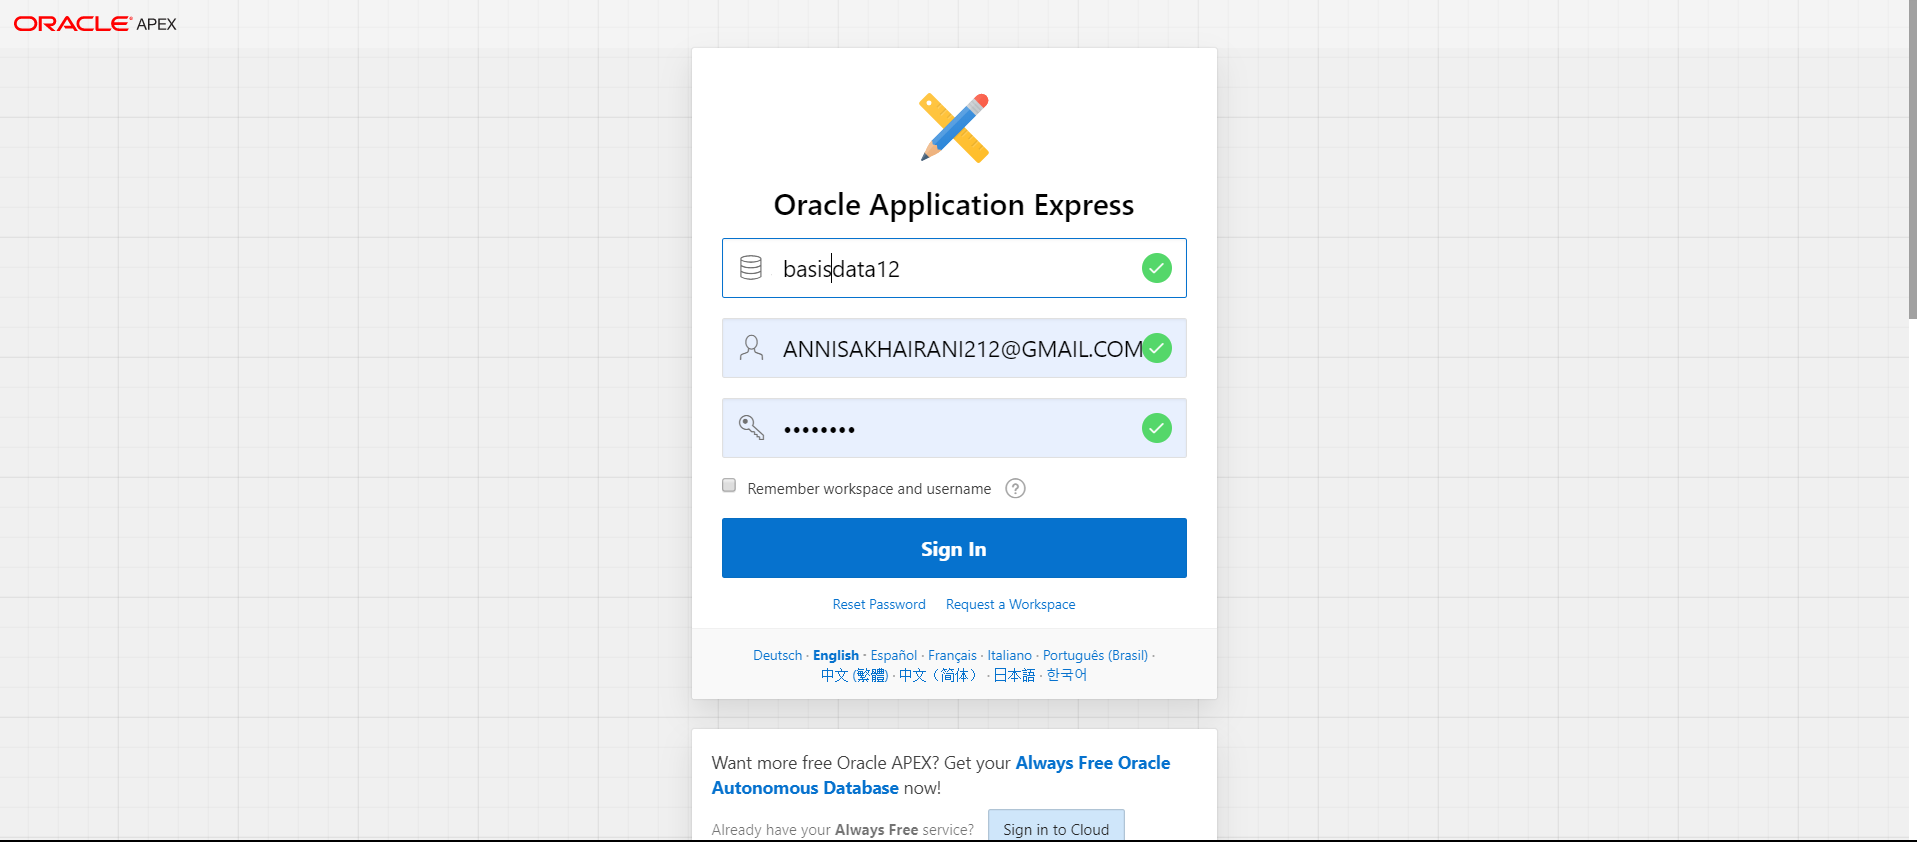
\includegraphics[width=10cm]{figure/1.PNG}}
\end{figure}
\newpage \begin{enumerate}
    \item Jika kalian sudah menginstall aplikasi oracle apex ataupun sudah mendaftar di oracle apex online makan akan masuk ke dalam aplikasi oracle apex.
    \item Setelah selesai kita pilih sql workshop dan pilih sql command. Sql command digunakan untuk mengetikkan query yang akan kita gunakan.
    \item Langkah selanjutnya adalah pembuatan database yang dimulai dengan membuat suatu table, Disini saya membuat aplikasi tentang Klinik Dahlia yang terdapat tiga tabel yaitu Dokter, Pasien, dan Obat. Query yang diinputkan di sql command seperti berikut :
\end{enumerate}
{Table Dokter}
Table Dokter mempunyai 6 kolom yaitu Kd Dokter, Kd Poli, Tgl Kunjungan, Kd User, Nm Dokter, SIP
\begin{center}
    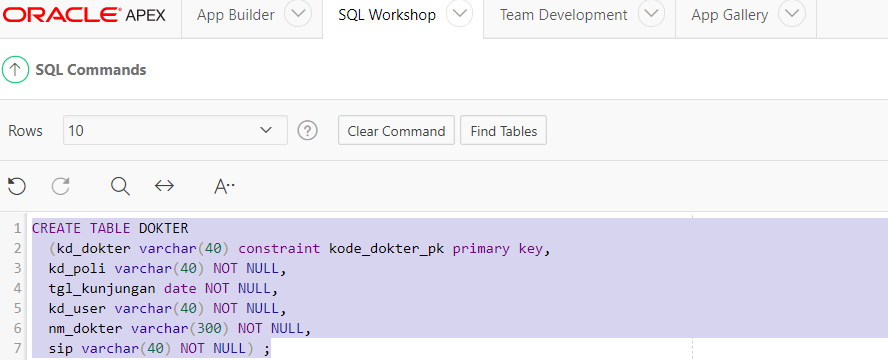
\includegraphics[width=10cm]{figure/dokter1aa.png}
\end{center}
{Table Pasien}
Table Pasien mempunyai 8 kolom yaitu No Pasien, Nm Pasien, J kel, Agama, Alamat, Tgl Lhr, Usia, No Tlp
\begin{center}
    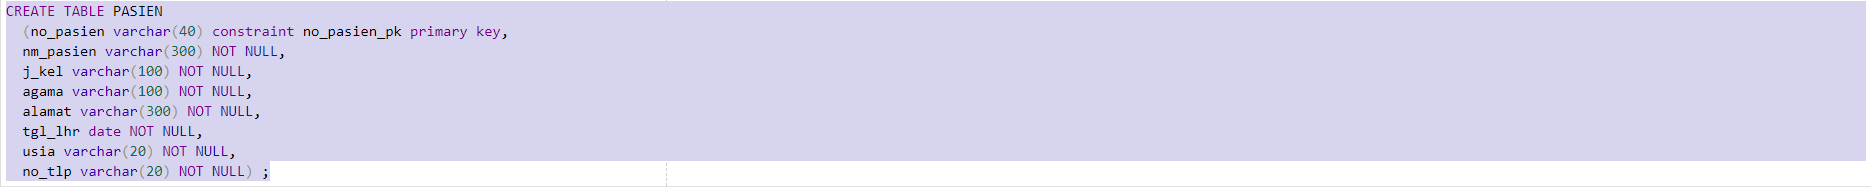
\includegraphics[width=10cm]{figure/pasien.PNG}
\end{center}
{Table Obat}
Table Obat mempunyai Kd Obat, Nm Obat, Jml Obat, Ukuran Varchar, Harga Varchar
\begin{center}
    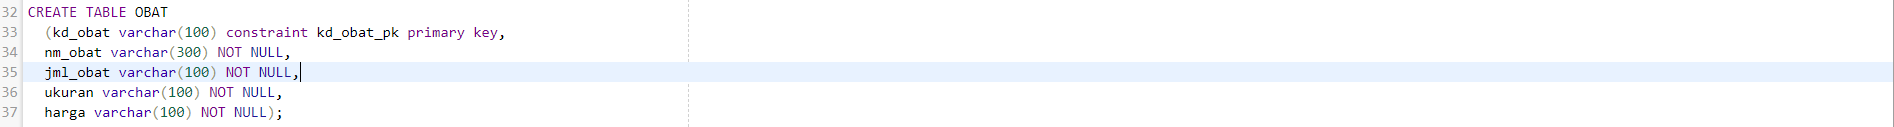
\includegraphics[width=10cm]{figure/obat.PNG}
\end{center}
\newpage \begin{enumerate}
    \item Setelah selesai membuat table maka selanjutnya adalah mengisi baris pada kolom table yang dinamakan (Insert) yang telah kita buat. Berikut adalah cara menambahkan baris pada kolom :
    
{Table Dokter}
Pada table dokter mempunyai  dua kolom maka baris yang dimasukkan juga sebanyak dua baris sesuai dengan jumlah kolom.
\begin{center}
    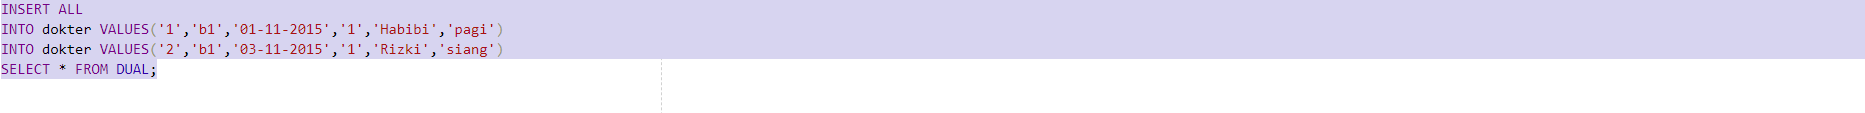
\includegraphics[width=10cm]{figure/insert1.PNG}
\end{center}
{Table Pasien}
Pada table pasien mempunyai lima kolom maka baris yang dimasukkan juga sebanyak lima baris sesuai dengan jumlah kolom
\begin{center}
    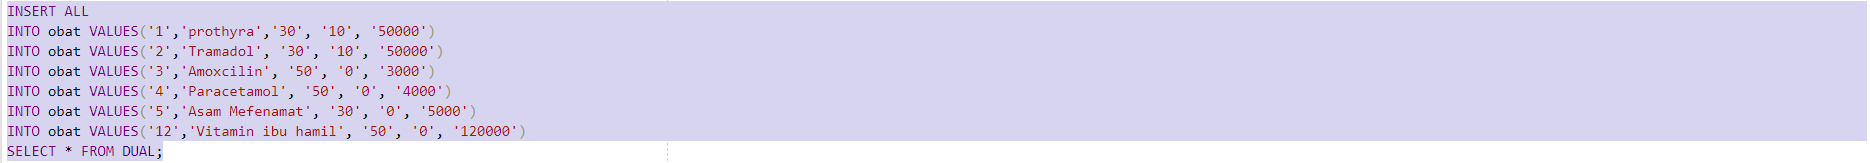
\includegraphics[width=10cm]{figure/insert2.PNG}
\end{center}
{Table Obat}
Pada table obat mempunyai enam kolom maka baris yang dimasukkan juga sebanyak enam baris sesuai dengan jumlah kolom
\begin{center}
    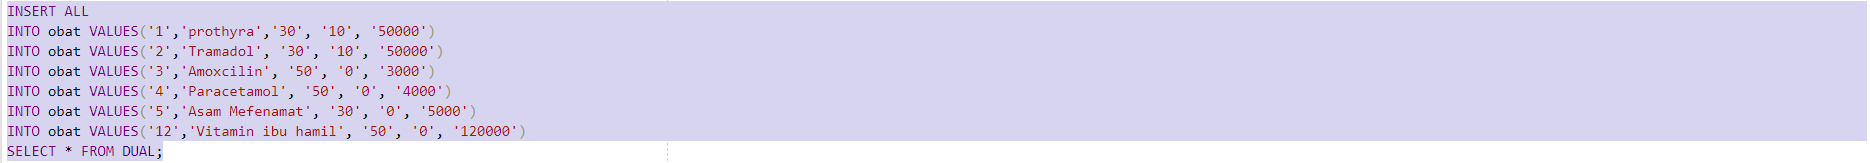
\includegraphics[width=10cm]{figure/insert3f.PNG}
\end{center}
{Table History Dokter}
Pada Table History Dokter digunakan untuk memanggil trigger yang akan digunakan, disini saya menggunakan table Dokter
\begin{center}
    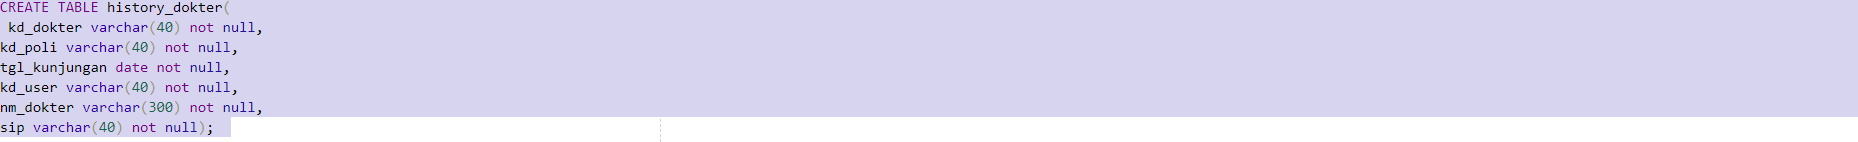
\includegraphics[width=10cm]{figure/dokter.PNG}
\end{center}
\item Setelah column dan baris diisi maka selanjutnya adalah pembuatan  fungsi trigger. Fungsi trigger adalah fungsi yang digunakan untuk menampilkan suatu data secara otomatis pada saat insert,delete dan update pada suatu table. Berikut ini merupakan triggers yang dibuat :
\begin{center}
    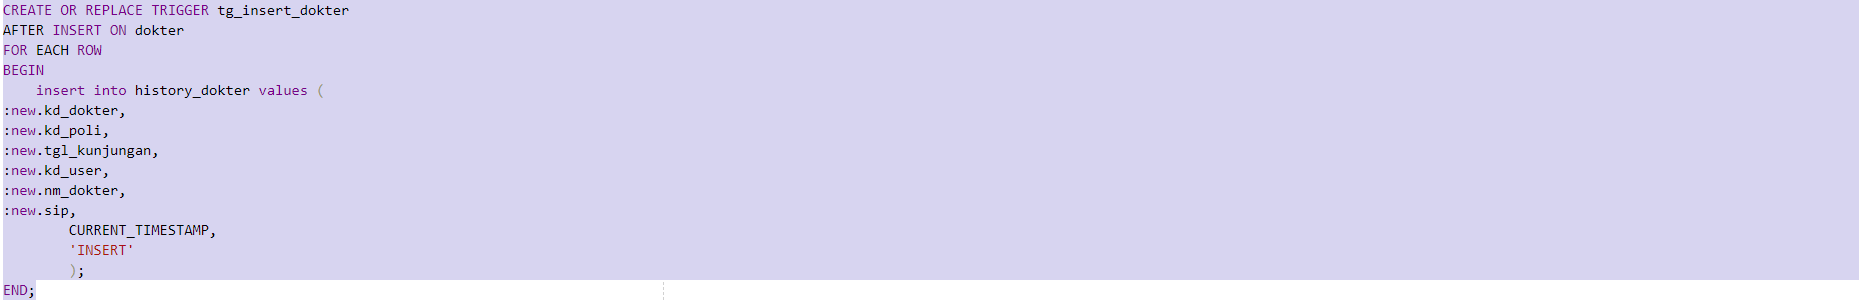
\includegraphics[width=10cm]{figure/insert.PNG}
    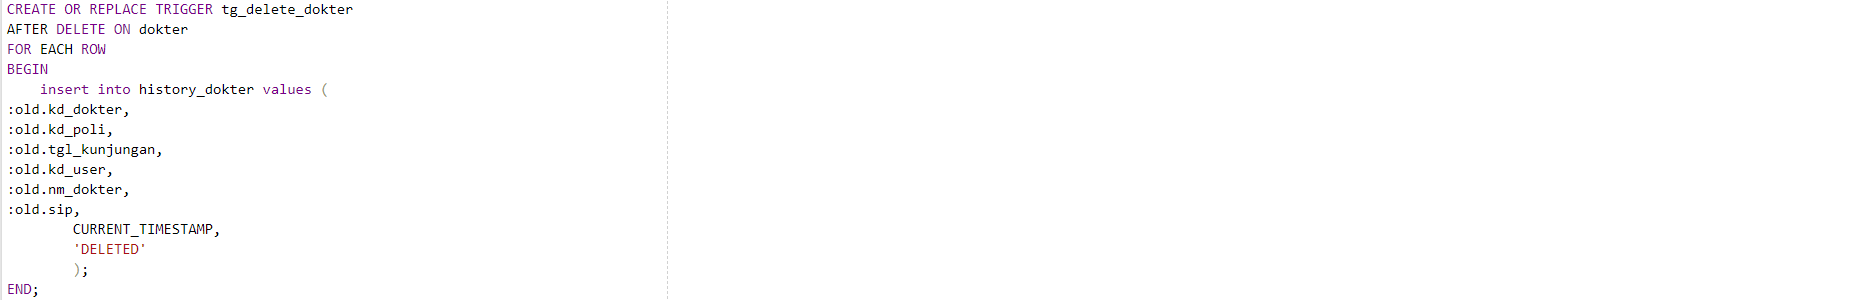
\includegraphics[width=10cm]{figure/delete.PNG}
    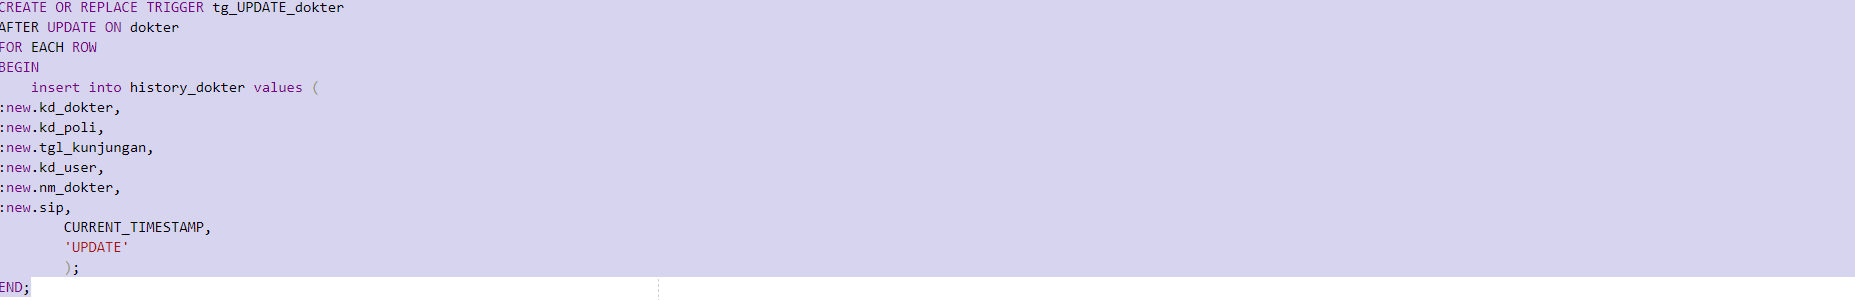
\includegraphics[width=10cm]{figure/update.PNG}
\end{center}
\item Setelah selesai pembuatan trigger ada tahapan pembuatan view pada aplikasi. View merupakan perintah untuk menggabungkan query join,innerjoin table dengan lebih sederhana.
\item Setelah selesai pembuatan trigger dan view selanjutnya kita bikin pembuatan sinonim. Sinonim digunakan untuk memanggil memanggil nama table dengan nama yang berbeda.
\item Setelah semuanya selesai, maka tahapan selanjutnya adalah pembuatan aplikasi dengan memilih app builder
\begin{center}
    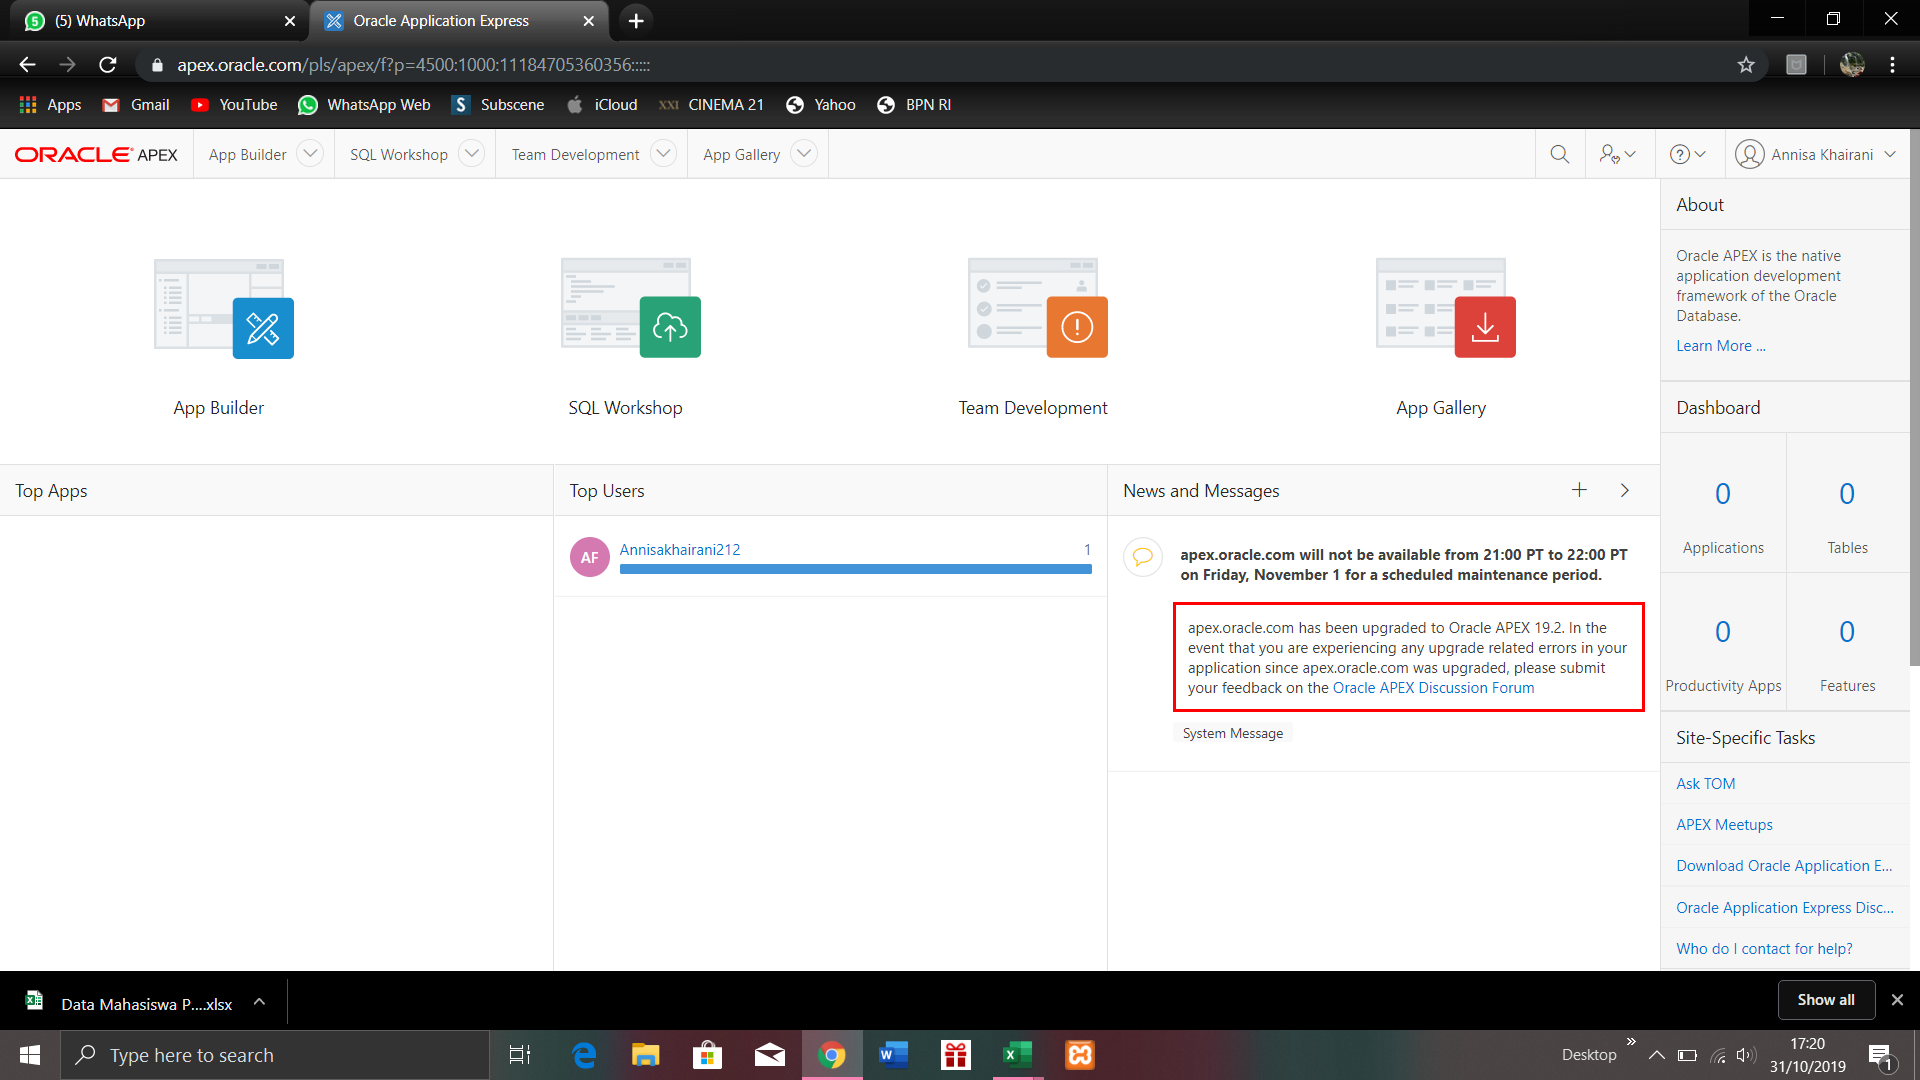
\includegraphics[width=10cm]{figure/3.png}
\end{center}
\item setelah itu kita pilih create untuk membuat aplikasi yang baru dengan menggunakan data-data yang telah dibuat pada Oracle Apex
\begin{center}
    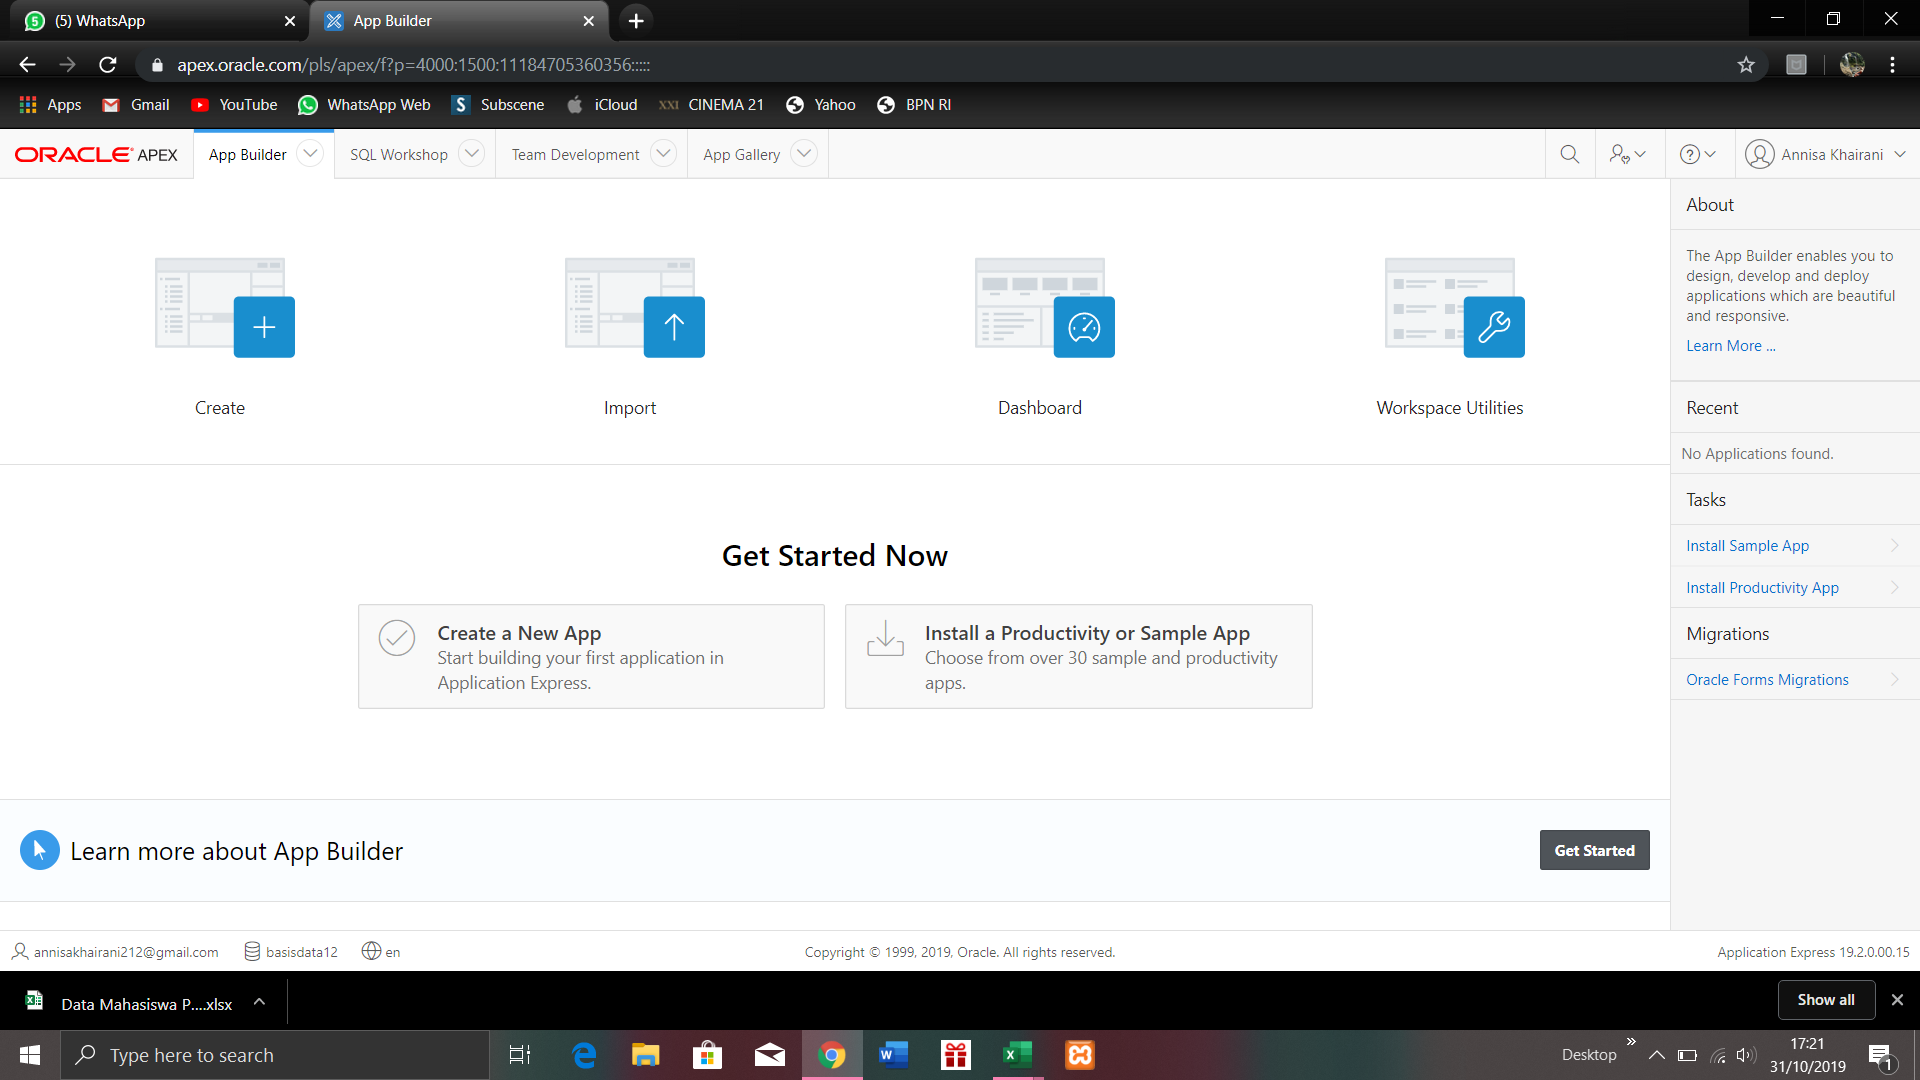
\includegraphics[width=10cm]{figure/4.png}
\end{center}
\item Setelah pilih create, kemudian kita pilih new application yang digunakan untuk membuat sebuah aplikasi yang akan kita gunakan
\begin{center}
    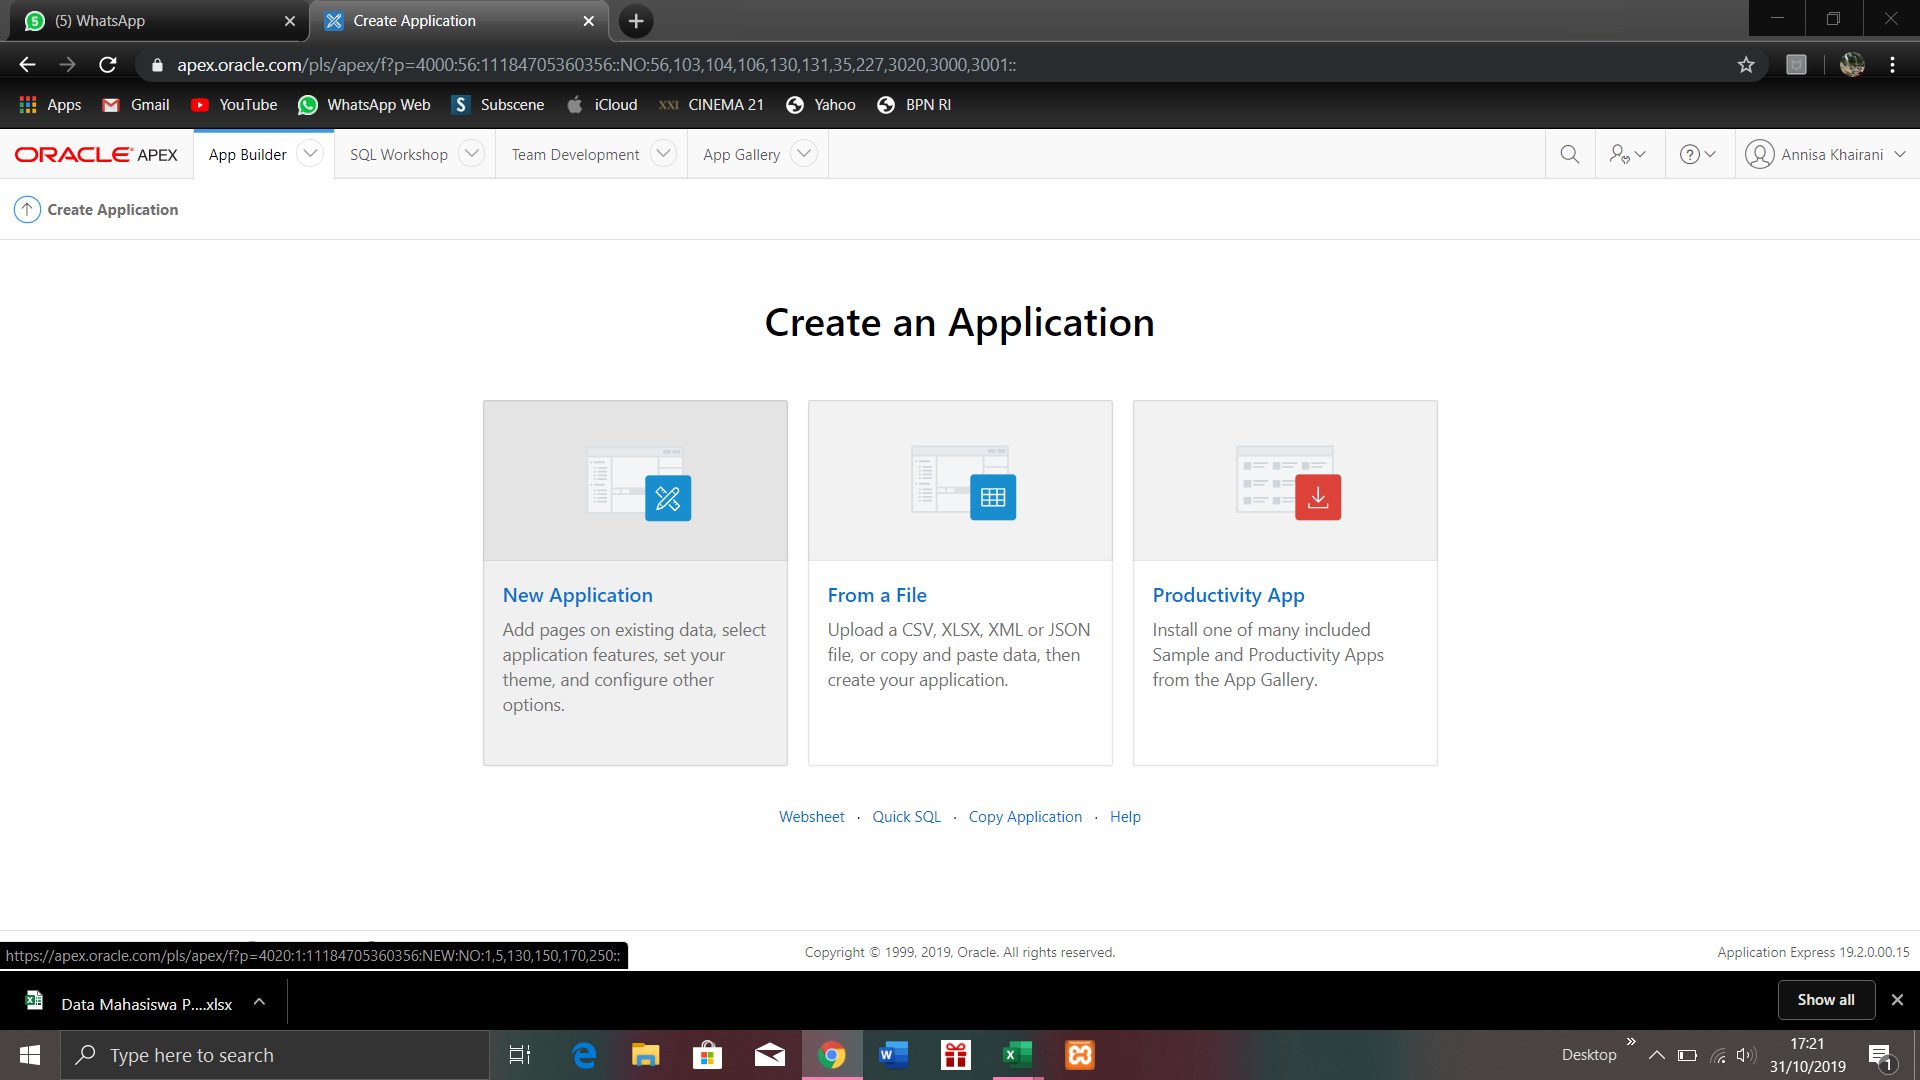
\includegraphics[width=10cm]{figure/5.png}
\end{center}
\item Setelah itu buatlah nama aplikasi yang akan dibuat,lalu pilih add page untuk memilih page yang akan digunakan untuk membuat sebuah aplikasi.
\begin{center}
    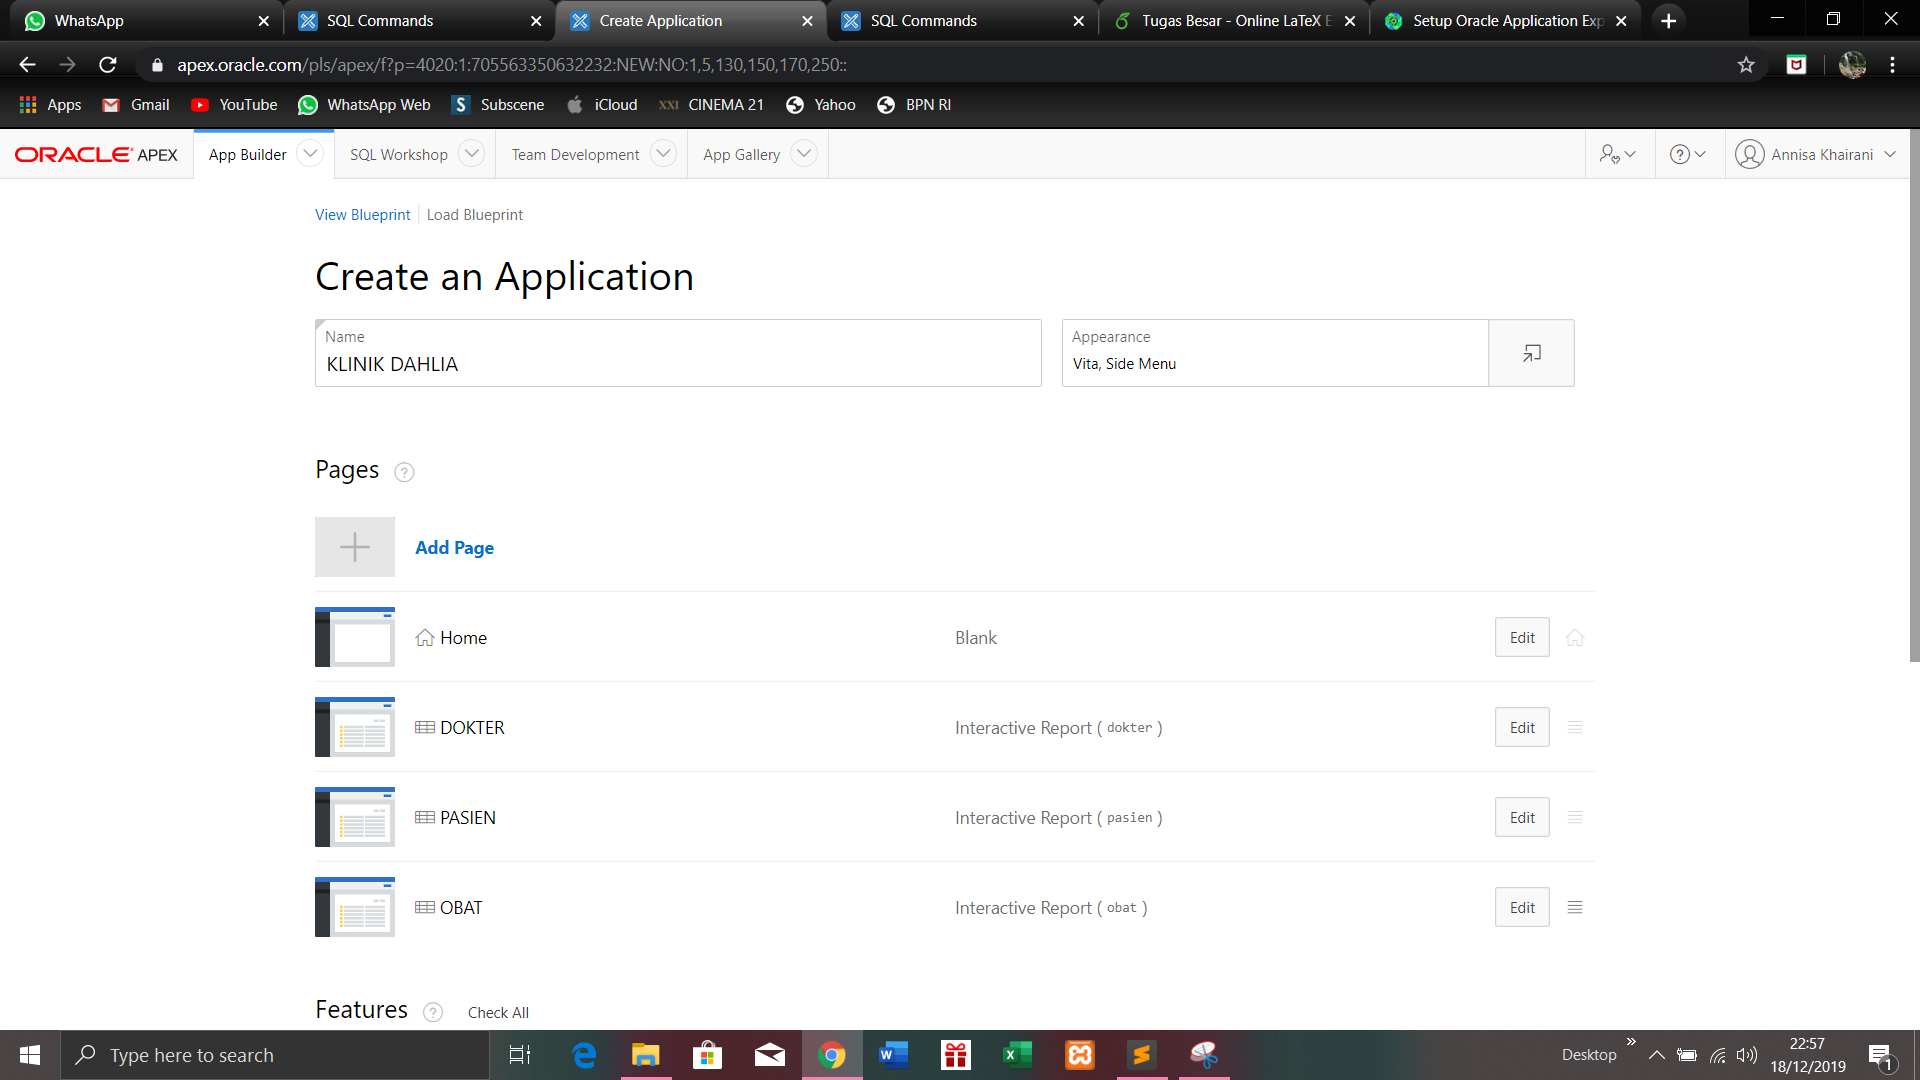
\includegraphics[width=10cm]{figure/209.png}
\end{center}
\item Kemudian pilih interactive report untuk page aplikasi yang dibuat
\begin{center}
    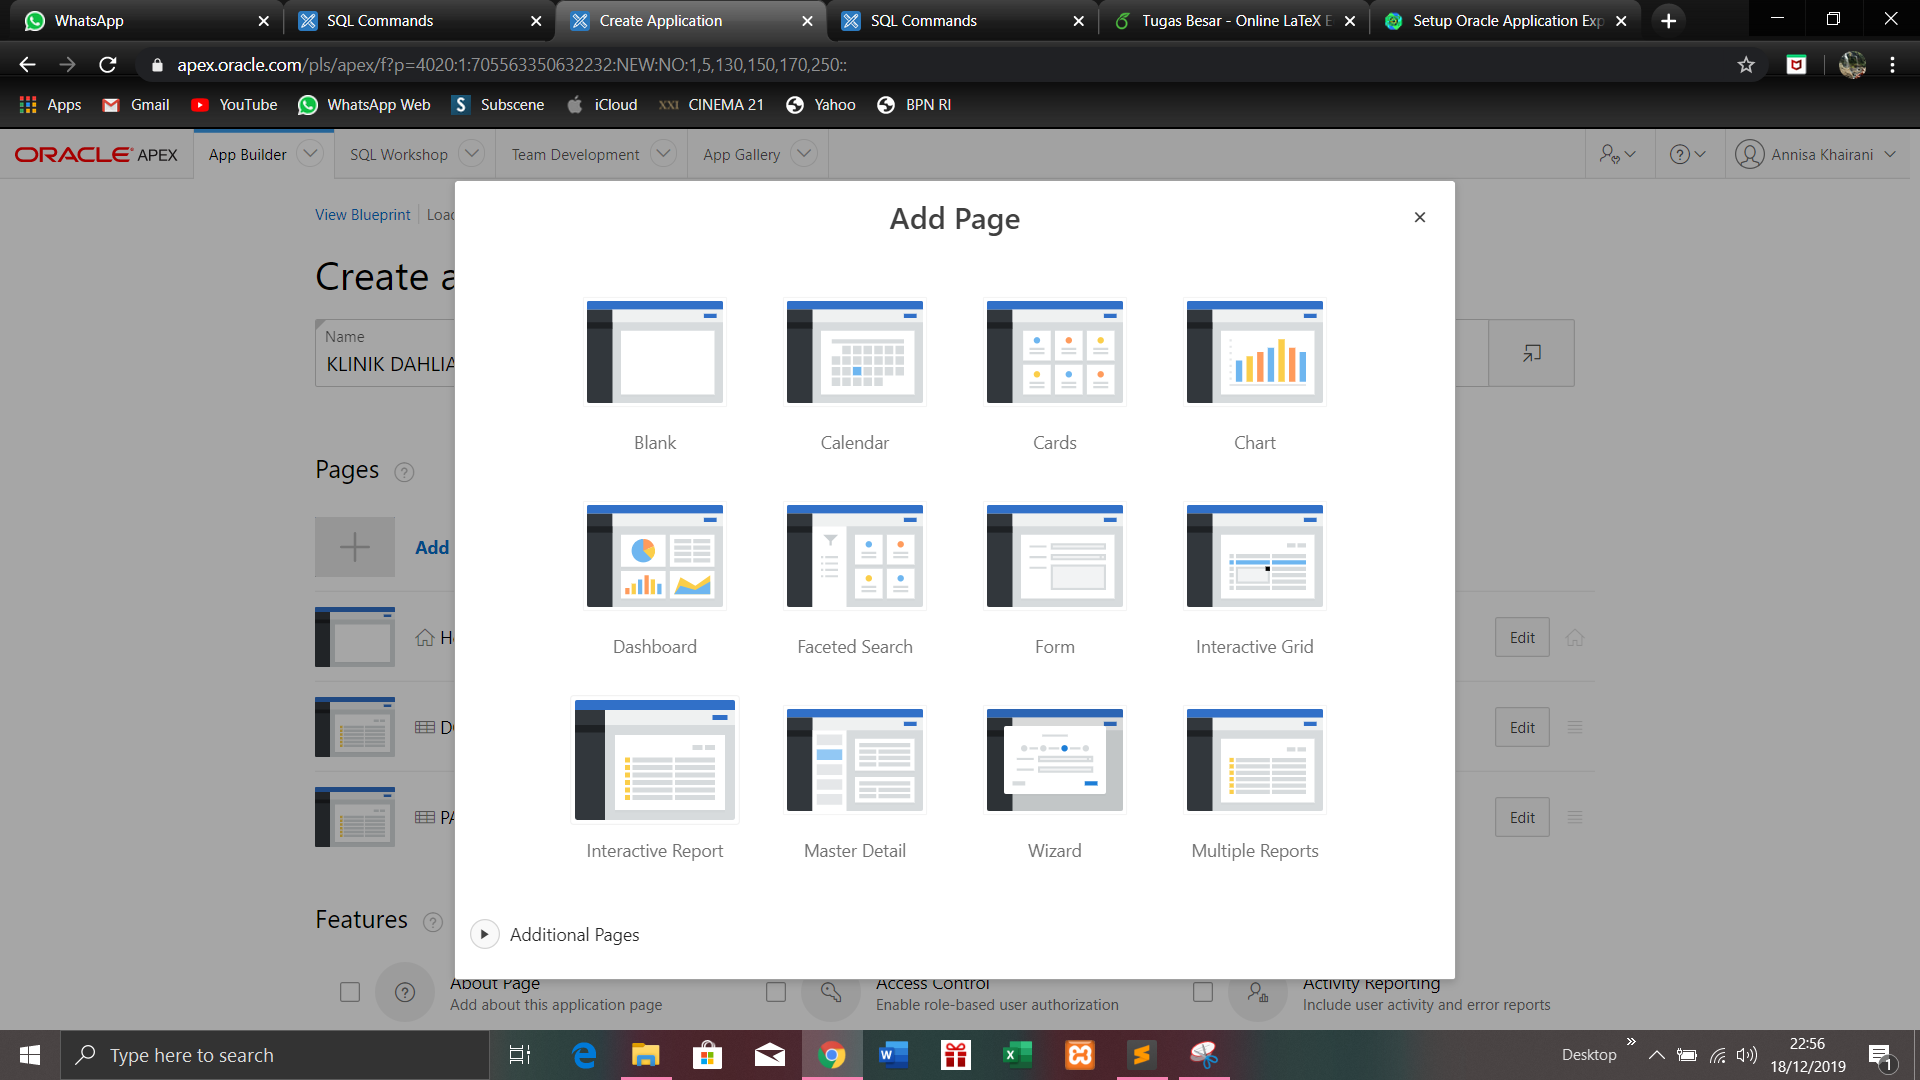
\includegraphics[width=10cm]{figure/207.png}
\end{center}
\item setelah itu isi page nama nya dengan Dokter yang merupakan table pertama pada aplikasi. Pilih table Dokter pada table or view lalu add page
\begin{center}
    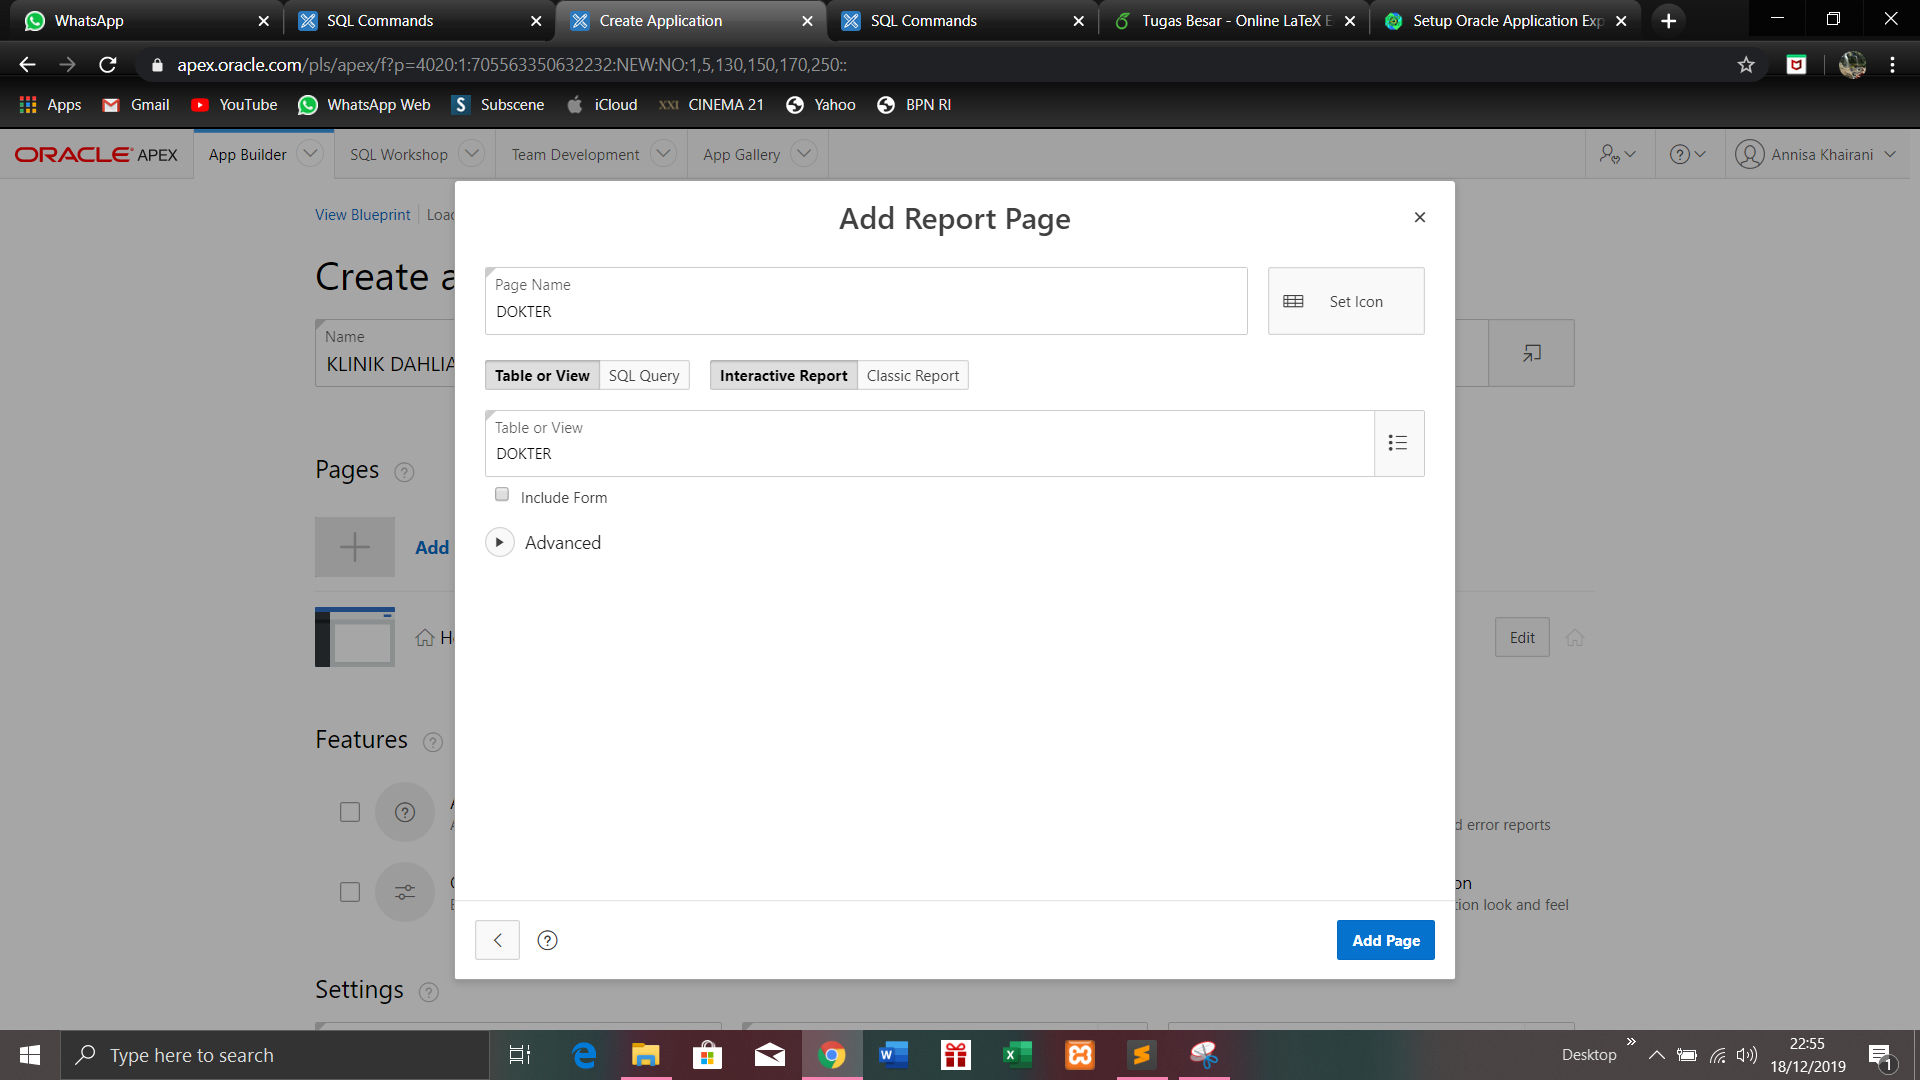
\includegraphics[width=10cm]{figure/205.png}
\end{center}
\item Setelah itu lakukan hal yang sama dengan pilih add page dan pilih page intercative report lalu isi name page dengan Pasien, dan Obat secara bergantian. Kemudian pilih table atau view table yang yang telah dibuat yaitu Dokter, Pasien, dan Obat  secara bergantian. Lalu kita tekan add page.
\begin{center}
    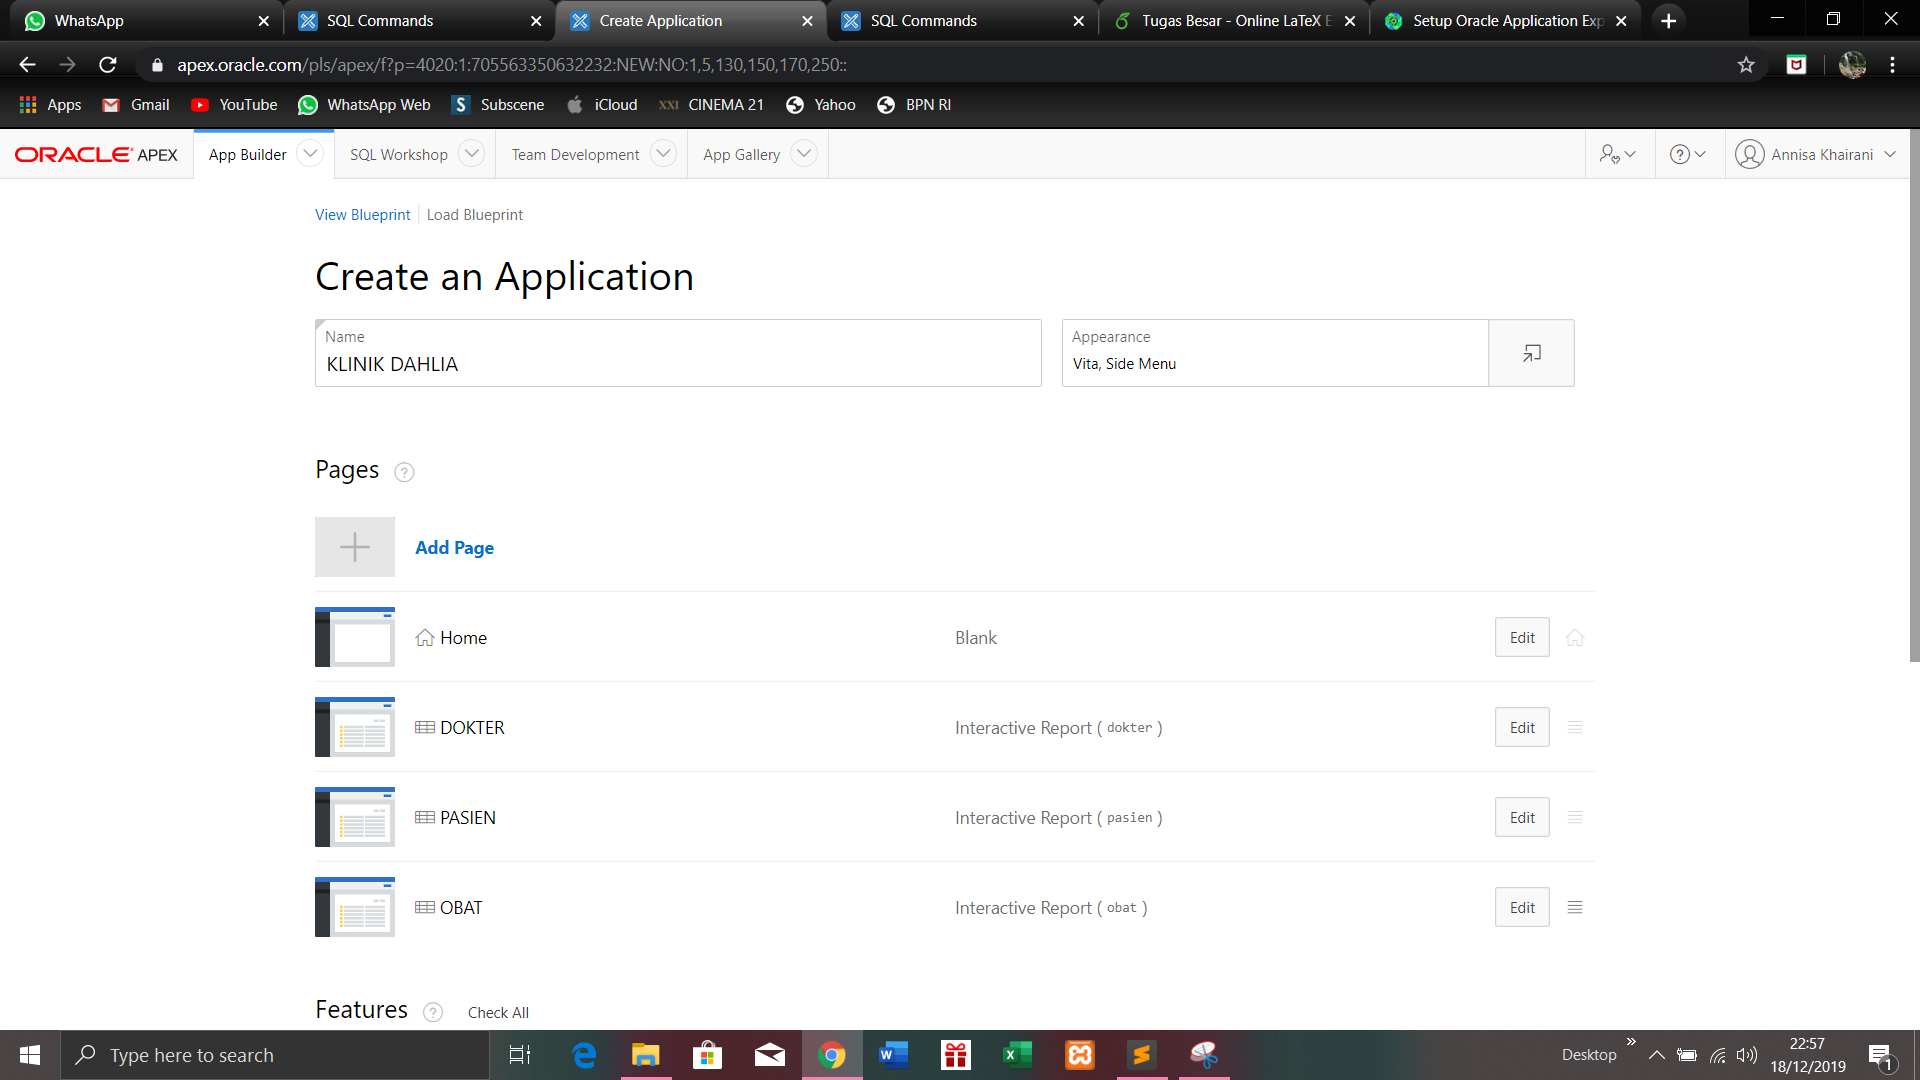
\includegraphics[width=10cm]{figure/2091.png}
\end{center}
\item setelah semuanya di add page maka pada features di cek all. Maka setelah itu create application. Tungga hingga selesai.
\begin{center}
    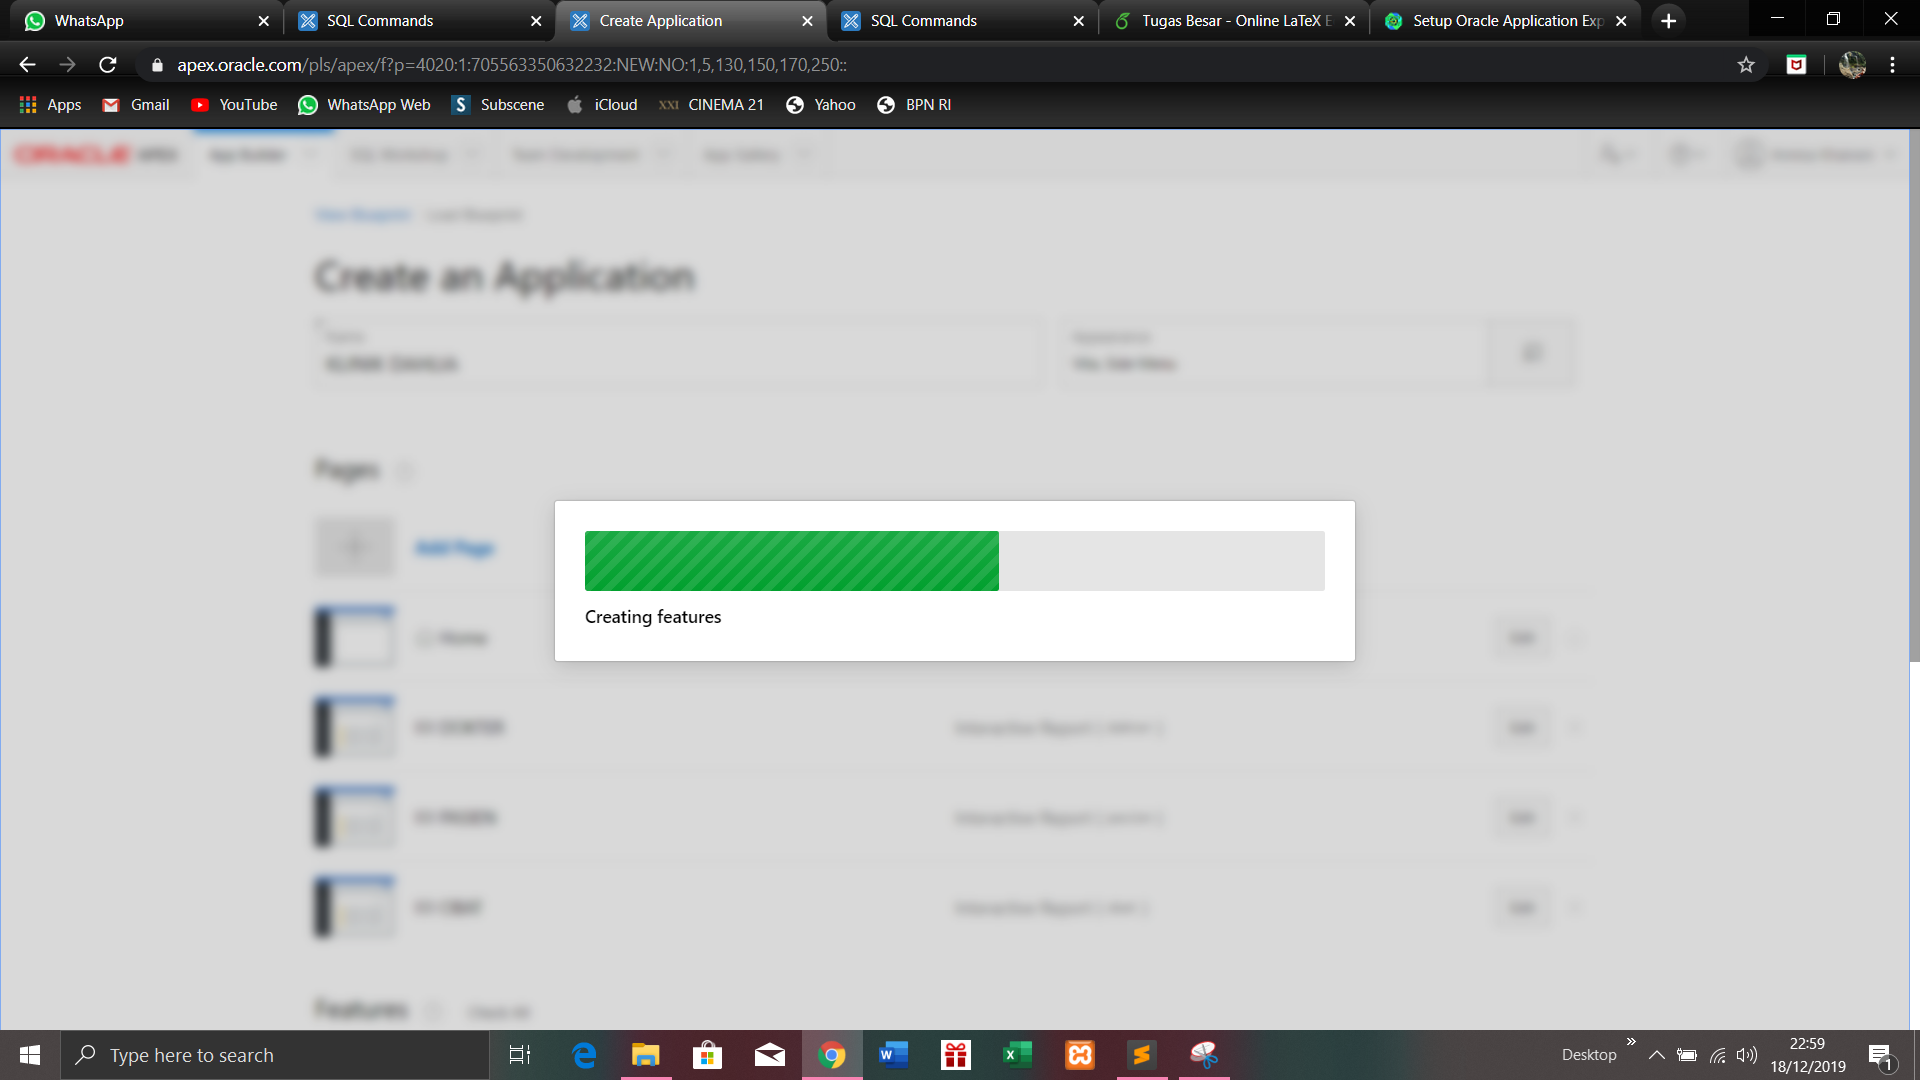
\includegraphics[width=10cm]{figure/210.png}
\end{center}
\item Kemudian setelah selesai kita pilih run application untuk melihat hasil aplikasi yang sudah di buat dan masukkan username dan password untuk melihat aplikasi yang telah dibuat. Lalu sign in
\begin{center}
    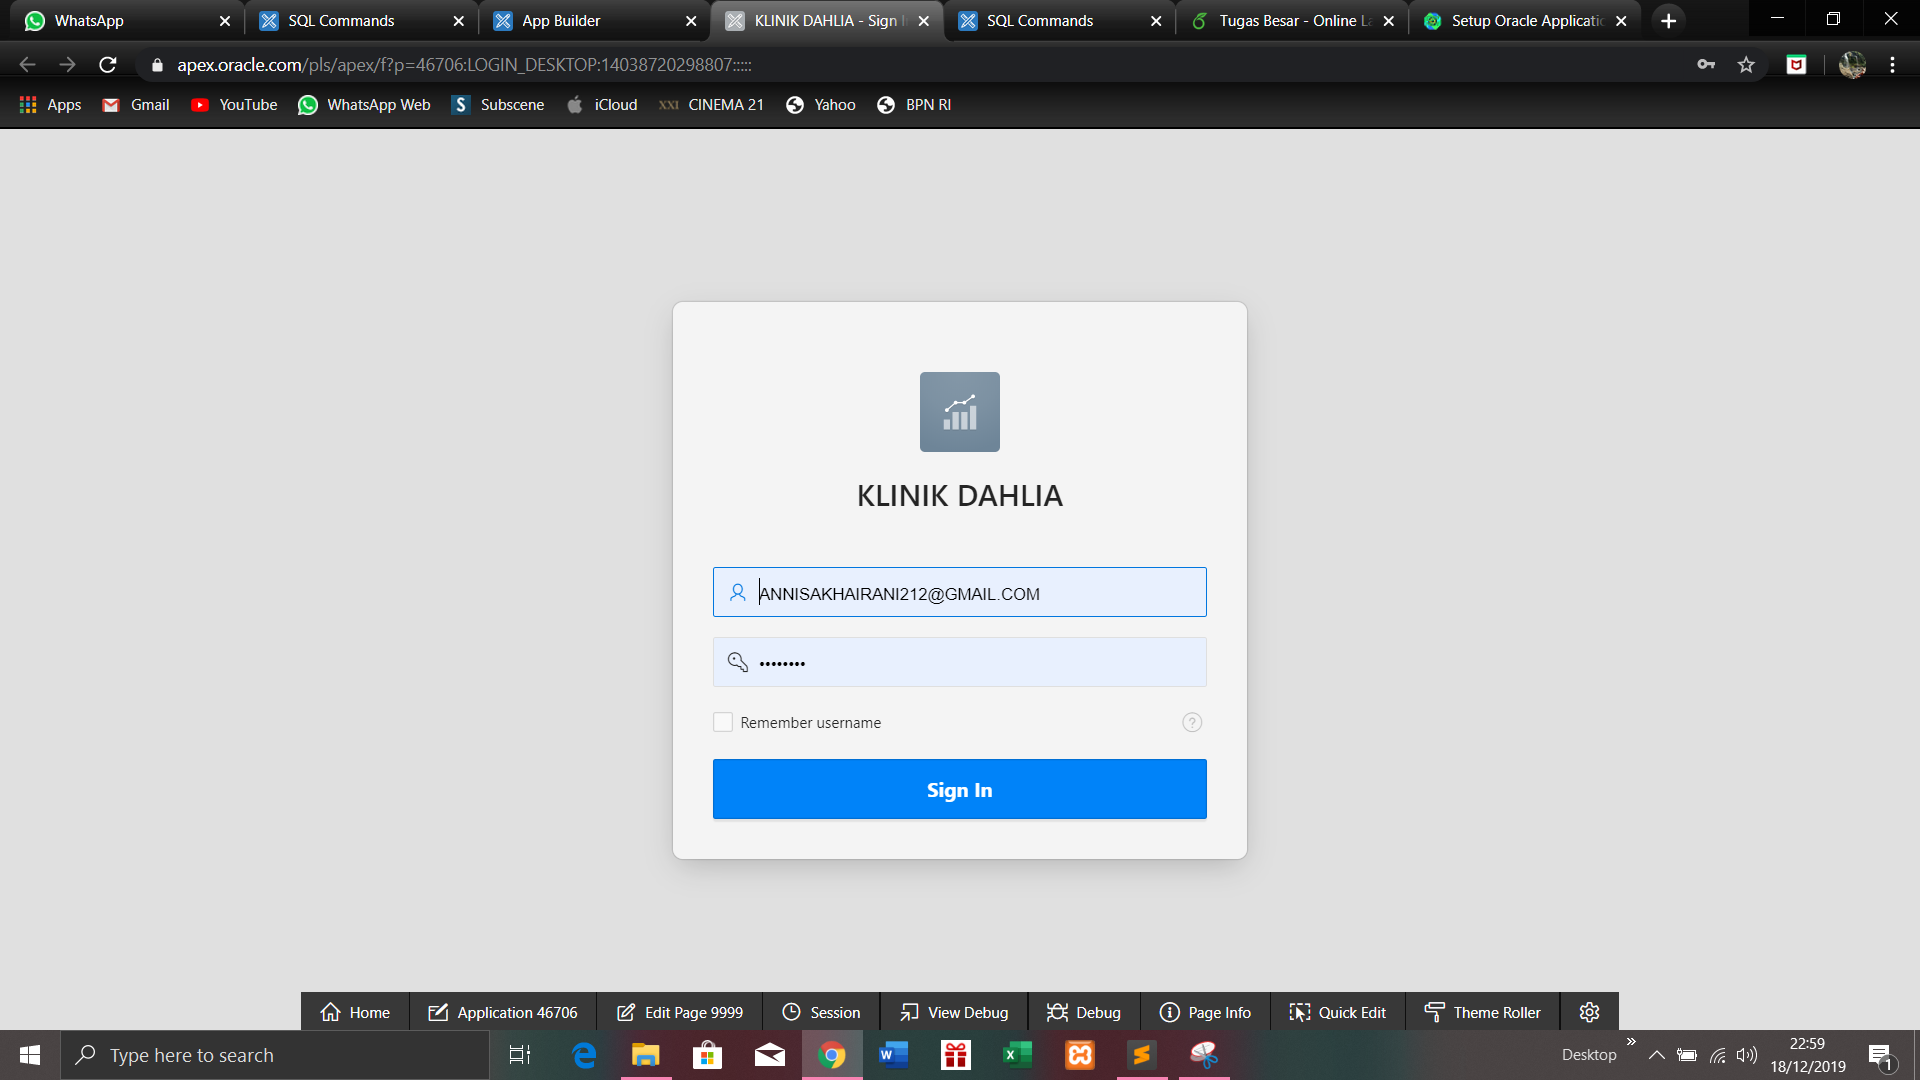
\includegraphics[width=10cm]{figure/211.png}
\end{center}
\item Maka aplikasi data Klinik Dahlia sudah selesai dibuat dan ini hasilnya
\begin{center}
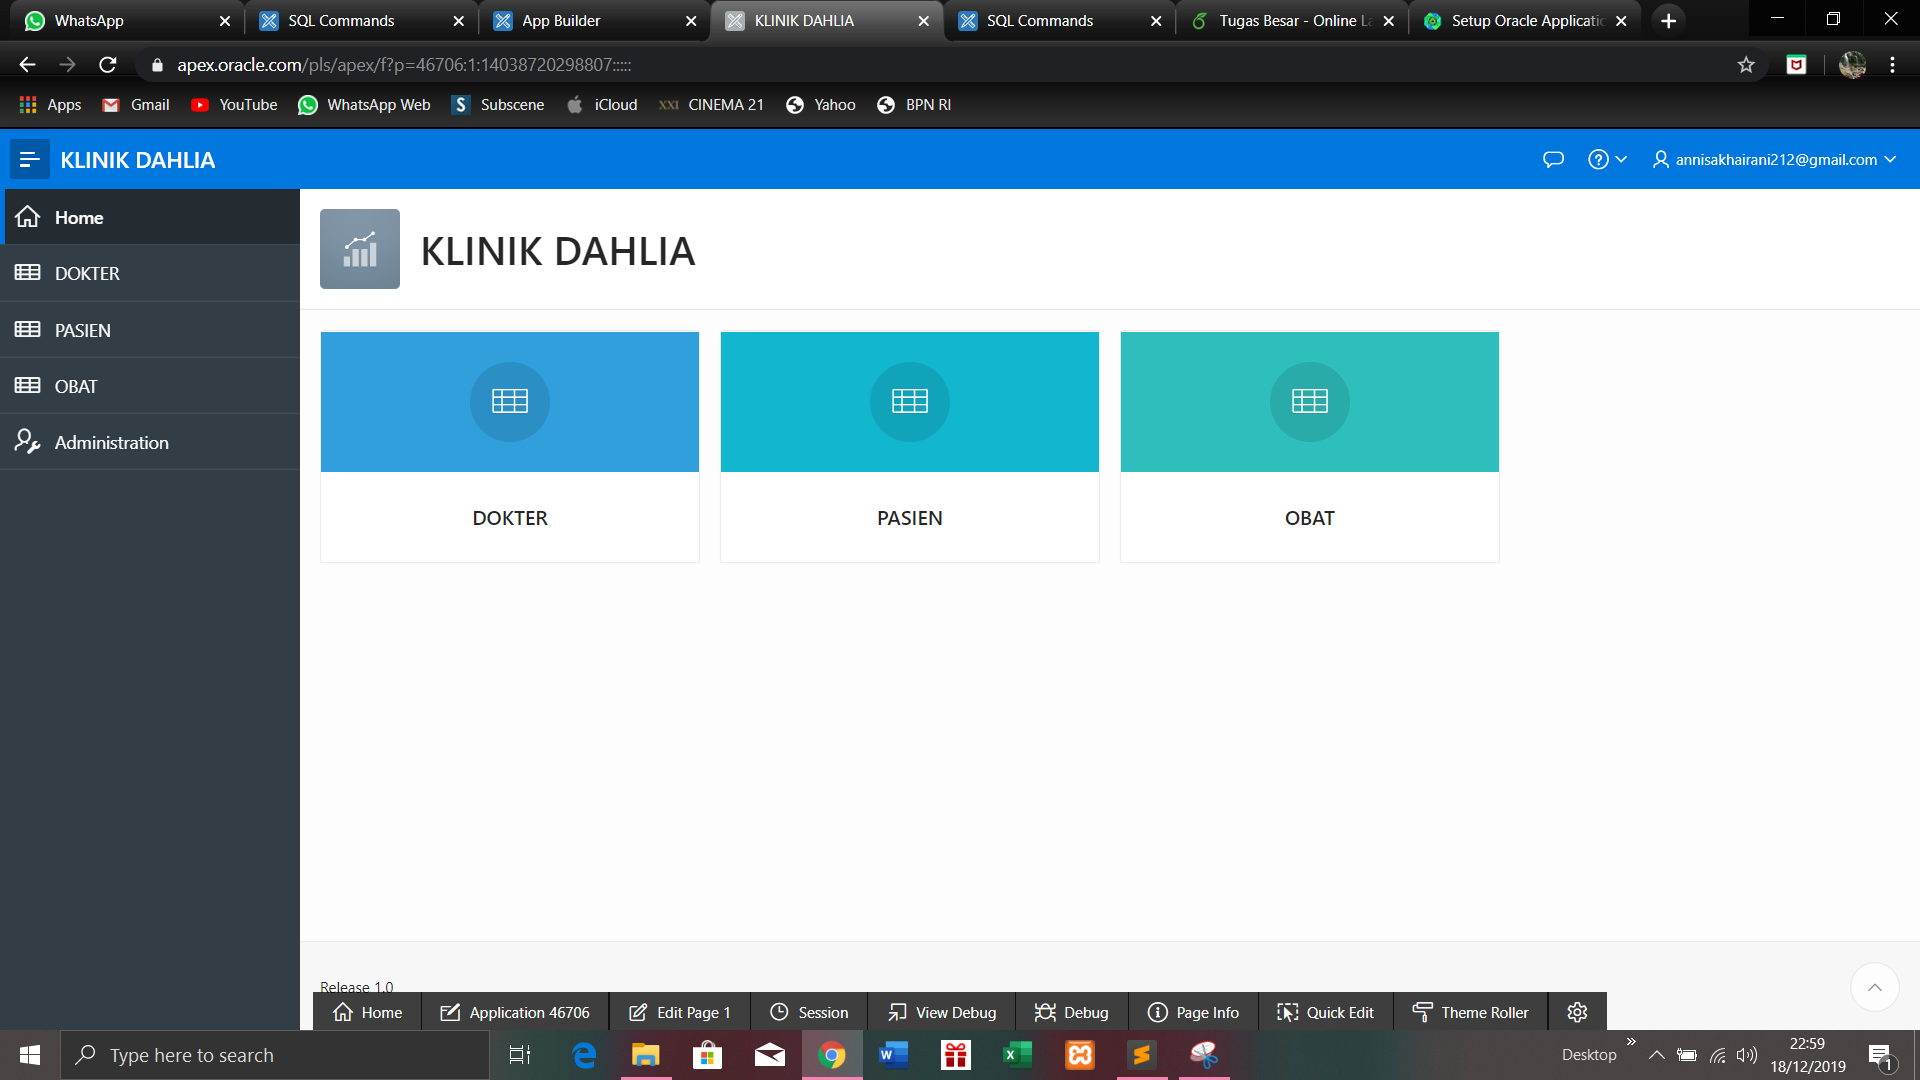
\includegraphics[width=10cm]{figure/212.png}
\end{center}
\end{enumerate}

\end{document}
